%% 
%% Copyright 2007, 2008, 2009 Elsevier Ltd
%% 
%% This file is part of the 'Elsarticle Bundle'.
%% ---------------------------------------------
%% 
%% It may be distributed under the conditions of the LaTeX Project Public
%% License, either version 1.2 of this license or (at your option) any
%% later version.  The latest version of this license is in
%%    http://www.latex-project.org/lppl.txt
%% and version 1.2 or later is part of all distributions of LaTeX
%% version 1999/12/01 or later.
%% 
%% The list of all files belonging to the 'Elsarticle Bundle' is
%% given in the file `manifest.txt'.
%% 

%% Template article for Elsevier's document class `elsarticle'
%% with numbered style bibliographic references
%% SP 2008/03/01

\documentclass[final,12pt]{elsarticle}

%% Use the option review to obtain double line spacing
%% \documentclass[authoryear,preprint,review,12pt]{elsarticle}

%% Use the options 1p,twocolumn; 3p; 3p,twocolumn; 5p; or 5p,twocolumn
%% for a journal layout:
%% \documentclass[final,1p,times]{elsarticle}
%% \documentclass[final,1p,times,twocolumn]{elsarticle}
%% \documentclass[final,3p,times]{elsarticle}
%% \documentclass[final,3p,times,twocolumn]{elsarticle}
%% \documentclass[final,5p,times]{elsarticle}
%% \documentclass[final,5p,times,twocolumn]{elsarticle}

%% For including figures, graphicx.sty has been loaded in
%% elsarticle.cls. If you prefer to use the old commands
%% please give \usepackage{epsfig}

%% The amssymb package provides various useful mathematical symbols
\usepackage{amssymb}

\usepackage{xeCJK}
\usepackage{subfig}
\linespread{1.2}

%% The amsthm package provides extended theorem environments
%% \usepackage{amsthm}

%% The lineno packages adds line numbers. Start line numbering with
%% \begin{linenumbers}, end it with \end{linenumbers}. Or switch it on
%% for the whole article with \linenumbers.
%% \usepackage{lineno}

\journal{CSP2016-期末论文}

\begin{document}

\begin{frontmatter}

%% Title, authors and addresses

%% use the tnoteref command within \title for footnotes;
%% use the tnotetext command for theassociated footnote;
%% use the fnref command within \author or \address for footnotes;
%% use the fntext command for theassociated footnote;
%% use the corref command within \author for corresponding author footnotes;
%% use the cortext command for theassociated footnote;
%% use the ead command for the email address,
%% and the form \ead[url] for the home page:
%% \title{Title\tnoteref{label1}}
%% \tnotetext[label1]{}
%% \author{Name\corref{cor1}\fnref{label2}}
%% \ead{email address}
%% \ead[url]{home page}
%% \fntext[label2]{}
%% \cortext[cor1]{}
%% \address{Address\fnref{label3}}
%% \fntext[label3]{}

\title{Sandboxing 相关技术研究与思考}

%% use optional labels to link authors explicitly to addresses:
%% \author[label1,label2]{}
%% \address[label1]{}
%% \address[label2]{}

\author{尹至达}
\author{高策}

\address{上海交通大学软件学院}

\begin{abstract}

目前,互联网上的攻击越来越频繁,攻击者会通过各种攻击方式,以达到获取系统高权限,读取敏感数据等等攻击目的。沙箱作为一个用来隔离程序执行环境,使得程序在一个低权限的,高度隔离的环境中执行的技术,受到了越来越多的关注。本文以一个现代的浏览器为出发点,介绍了两类沙箱技术在其中的应用与体现,进而总结对比各种沙箱实现的特点,并且在最后对沙箱技术下一步的研究方向提出了看法。

\end{abstract}

\begin{keyword}

Sandboxing \sep System Call Interposition \sep Capabilities \sep Software-based Fault Isolation

\end{keyword}

\end{frontmatter}

%% \linenumbers

%% main text
\section{引言}
\label{s:introduction}

随着网络全球化的发展,网络安全进入了大众视野,成为一个越来越引人注目的议题。互联网在提供给用户以便利的同时,也对隐私安全提出了新的挑战。这样的问题存在于各种平台上,攻击者会将诸如木马、病毒、恶意软件等等内容发布到被攻击者的终端上 \cite{miwa}。虽然现在的操作系统上的安全措施已经足够强大到防止绝大多数的攻击,但是用户总是期望更加安全的环境。而沙箱是一种非常实用的安全机制,通过引入沙箱技术,程序可以在隔离的环境中运行,使得程序的运行不会影响操作系统,同时操作系统也不会影响到程序。在传统的操作系统的抽象中,用户的应用对于系统各种资源的使用都是无限制的,而沙箱技术是对其运行时环境的隔离 \cite{sandbox}。

\begin{figure*}
\centering
\subfloat[第一类沙箱]{
\label{fig:t1sb}
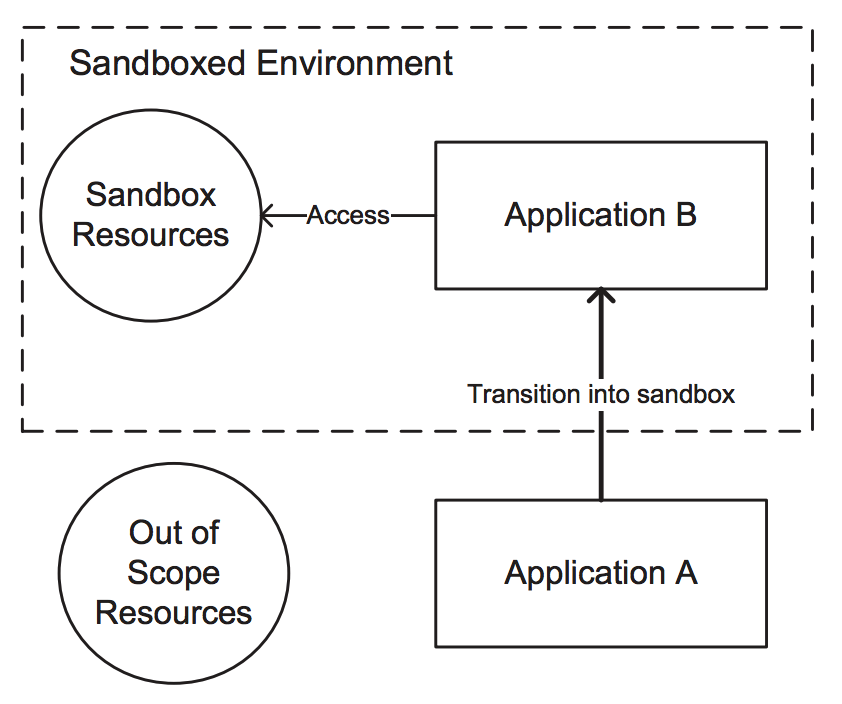
\includegraphics[width=0.4\linewidth]{imgs/type-1-sandbox.png}
}
\subfloat[第二类沙箱]{
\label{fig:t2sb}
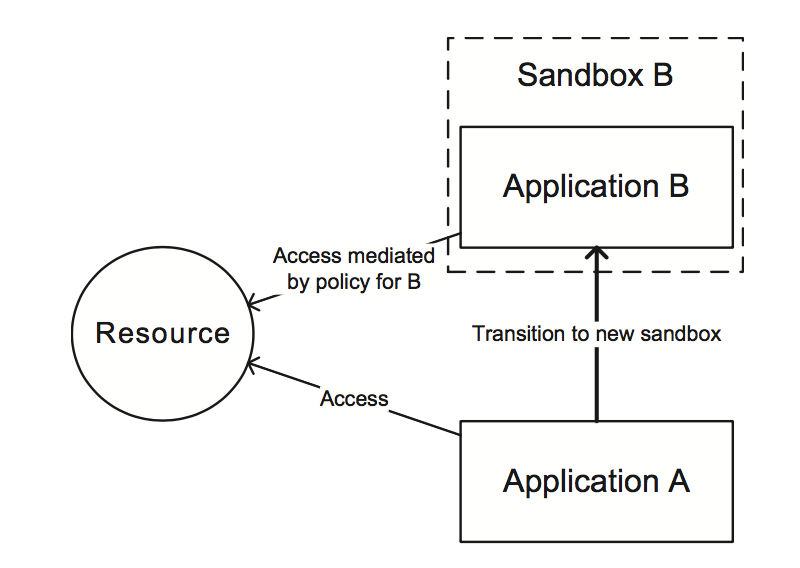
\includegraphics[width=0.4\linewidth]{imgs/type-2-sandbox.png}
}
\caption{沙箱分类}
\end{figure*}

沙箱技术大致可以被分为两类,其中第一类是基于隔离的沙箱,该类型的沙箱将应用的执行环境从操作系统中隔离出来,形成一个独立的执行环境。图 \ref{fig:t1sb} 展示了一个经典的基于隔离的沙箱模型。一个应用程序会在启动另一个应用程序之前先启动应用程序的沙箱,然后在沙箱内运行该应用程序,沙箱内的应用程序只能访问到沙箱内的资源。广为人知的虚拟机,容器,和传统意义上的沙箱都是这一类的沙箱模型。

第二类是基于规则的沙箱,该类型的沙箱并不是完全关注于对于应用程序的隔离上,而是用规则的方式控制每个应用的权限,基于规则的沙箱之间可以分享操作系统的逻辑资源。图 \ref{fig:t2sb} 展示了第二类的沙箱模型,不同于基于隔离的沙箱模型的地方在于,基于规则的沙箱模型并没有实现完全的资源隔离,而是对于每个应用,有不同的限制策略,通过强制应用限制策略来保证资源的访问权限受控 \cite{schreuders}。

由于篇幅限制,本文不能面面俱到地对各种沙箱技术都予以介绍,为了保证深度,本文选取第一类沙箱中的 Software-based Fault Isolation,以及第二类沙箱中的 System Call Interposition 和 Capabilities,来介绍沙箱技术的应用场景与实现,以及各自的优缺点,并在文末展开对各种技术的实现原理和潜在研究点的讨论。

\section{威胁模型}
\label{s:threat_model}

目前在互联网上,不受信任的应用的数量正在快速增长,让不受信任的应用程序能够更好地运行在系统中,是一件相当困难的事情。这些不受信用的应用程序可能隐藏有带有攻击意图的代码,它们获取操作系统高权限、读取文件系统中的敏感数据(比如密码、照片、文档等)、植入广告、导致系统崩溃等等。而攻击手段有很多,其中包括代码注入、Cross Site Scripting(CSS)、缓冲区溢出、Return-oriented programming(ROP) 等等 \cite{miwa}。	

传统的操作系统并没有很好地解决这方面的问题,在隔离方面,仅仅依靠运行时的简单隔离是不够的。新的趋势使得操作系统应该在处理器,内存等硬件层面和进程,文件系统等软件层面进行更加细致的隔离和容错。这也是沙箱技术关注的焦点。不同的沙箱技术针对的威胁模型都是不一样的,但是它们在宏观上都有一个共同点:防止不受信任的应用程序可以随意访问地操作系统或者底层的硬件。

\section{Sandboxing 相关技术以及使用场景}
\label{s:implementation}

为了能够深入浅出地进行介绍,方便理解,本节将以一个现代的浏览器作为应用场景进行切入,在浏览器上,沙箱有着非常多的应用:

\begin{itemize}
\item
网页应用,现代的浏览器会在沙箱中运行你打开的网页代码。诸如 Javascript 之类的网页代码在浏览器的沙箱中只有有限的权限,它们并不能直接与文件系统等等进行交互,因此 Javascript 中的恶意代码的破坏性仅限于在沙箱内。
\item
浏览器插件,浏览器并不会直接将插件进程运行在操作系统上,而是会将其运行在一个沙箱进程中。比如 Adobe Flash 插件,就是如此。这样的隔离方式使得插件如同网页应用一样不能直接与操作系统进行交互,防止两者之间相互的攻击。
\item
各类下载内容的查看器,以 PDF 文件为例,浏览器下载的 PDF 文件会使用系统内的 PDF 阅读器打开,目前一些 PDF 阅读器正在使用沙箱技术来解析 PDF 文件,其中最有名的是 Adobe Reader。它运行在一个沙箱中,因此如果 PDF 文件中有恶意内容,也不会影响到操作系统。
\item
浏览器本身,浏览器是沙箱技术运用最广泛的桌面应用之一。浏览器不止将其请求的网页应用和插件等运行在容器中,浏览器本身也是运行在一个独立而隔离的沙箱中的。低权限的沙箱运行可以保证即使恶意内容破坏了网页应用所在的沙箱,也会被浏览器的沙箱所限制 \footnote{http://www.howtogeek.com/169139/sandboxes-explained-how-theyre-already-protecting-you-and-how-to-sandbox-any-program/}。
\end{itemize}

本节将介绍 System Call Interposition(SCI)、Software-based Fault Isolation(SFI) 和 Capabilities 等技术在浏览器中的体现。System Call Interposition(SCI) 通过对系统调用的跟踪和限制,来使得应用不可以调用一些敏感的系统调用,或者不能将敏感的参数传入到系统调用中。Software-based Fault Isolation(SFI) 更加关注如何在一个应用程序产生了故障后,不会影响到其他的应用程序,同时保证应用程序之间的数据和代码是不能被彼此访问到的。Capability Security Model(CSM)是一种区别于对服务提供者进行诸如Acccess Control List(ACL)的权限检查,而将权限检查绑定在被需要的实体上的一种设计理念 \footnote{http://wiki.c2.com/?CapabilitySecurityModel}。这是三种完全不同的思路,它们的目的都是隔离代码的运行环境,构建出一个高度隔离的,低特权级的沙箱环境。

\subsection{System Call Interposition(SCI)}
\label{ss:sci}

在浏览器中,有很多互联网上的内容是需要下载,然后使用本地的查看器打开的。比如 PDF 文件等,需要通过 Adobe Reader 等专用软件打开。但是下载的内容有可能是隐藏有恶意代码的,但是本地的查看器并不一定将其视为不可信的内容,因此下载的内容在被相应的查看器打开时,恶意代码可能会被错误地执行了。对 System Call Interposition(以下称为 SCI)的研究,起初的动机是如何限制打开浏览器下载内容的助手应用,希望能够限制助手应用本身进行系统调用的权限。它的思想是通过监控和审查应用程序进行的系统调用,保证其不能顺利进行系统不允许其进行的系统调用。SCI 的思想参考了 Unix 的最小特权原则,所有应用程序都应该被授予其需要的权限组成的最小集合。本节将以 Janus 和 Ostia 作为主要内容,介绍 SCI 的思想和实现。

\subsubsection{Janus}
\label{sss:janus}

Janus \cite{goldberg} 是 Goldberg 在 1996 年发表的论文,也是第一个成型的 SCI 系统实现,是这一领域奠基性的论文。Janus 最初的动机是限制助手应用的权限,其提出了几种可能的实现方法。其中包括:

\begin{itemize}
\item
在每个助手应用中单独地实现自己的安全保护。这是第一个被排除的选择,这样的实现会使得应用的实现变得更加复杂,而且应用的提供商未必有动力去实现完全的安全保护。而很多应用是闭源的,因此成本极大。从另一方面来讲,安全可以在更加底层的角度来实现。
\item
在操作系统中加入新的安全特性。所有的应用程序都是运行在操作系统之上的,因此只要在操作系统层面实现了安全策略,那所有的应用程序都会受益。但是 Janus 最后没有采取这样的方法,因为开发和维护这样的特性是需要修改内核的,很多用户不希望自己在添加安全保护的时候需要请系统管理员来为自己的操作系统打补丁。而且在内核中的修改是特别危险的,内核中的 bug 往往会造成更加严重的安全事故。
\item
使用已有的 reference monitor。传统操作系统中的 monolithic 的 reference monitor 不能保护应用程序不会被攻击,而只能保证攻击不会很快的传播。
\item
传统的网络防火墙。这样的思路实现起来会非常复杂,因为这样的一个过滤器或者代理需要支持所有的文件格式等等。
\end{itemize}

因此,在分析了现有的思路都不能满足需求后,Janus 的作者提出了一种新的思路,一种在用户态实现安全的方法。它的实现不要求修改操作系统和应用程序,而只是在用户态实现了一个 policy engine,进而对于每一个应用程序指定一个安全策略,由 policy engine 来保证安全策略会被应用在应用程序运行时。

\begin{figure*}
\centering
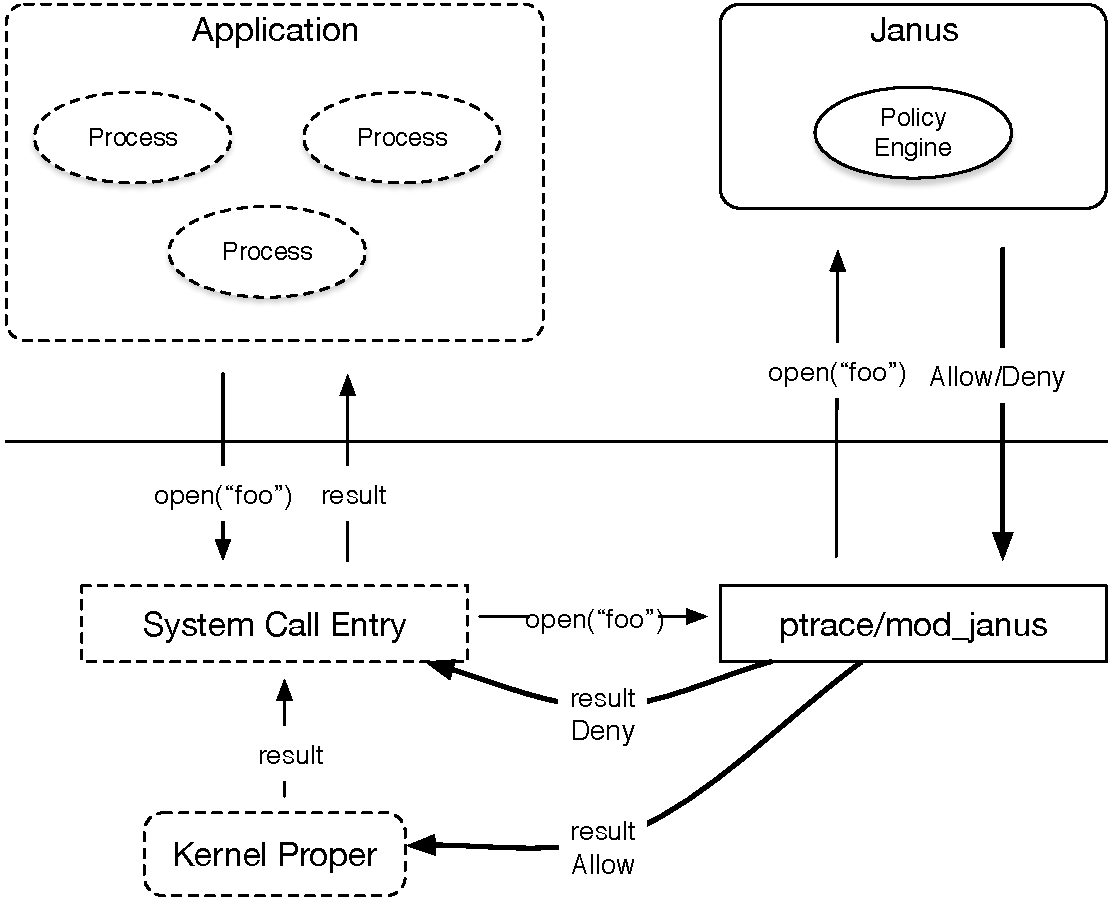
\includegraphics[width=0.7\linewidth]{imgs/janus}
\caption{Janus 架构图}
\label{fig:janus}
\end{figure*}

在设计架构时,Janus 主要考虑了三点:

\begin{itemize}
\item
安全,这也是最基本的原则。Janus 保证应用程序不能访问它没有权限访问的系统或者网络。为了更加地安全可靠,Janus 认同 "keep it simple" 的理念 \cite{keepitsimple}。Janus 认为只有简单的实现才能使得其更加安全。
\item
灵活,Janus 不仅可以做到在系统调用的粒度实现拦截与过滤,同时希望在更加细致的粒度,比如系统调用的参数等粒度上同样可以进行请求的拦截与过滤。
\item
可配置,Janus 应该用户针对不同的应用程序进行不同的策略定制。
\end{itemize}

为了实现上述三点,Janus 进行了如图 \ref{fig:janus} 所示的架构设计。其中由 Janus 负责实现的只有右上角的 policy engine,其他是由操作系统或者应用程序来实现的。当一个应用程序被启动时,Janus 会读取该应用程序的配置文件,随后会 fork 一个子进程,在子进程中运行应用程序,并且会调用 ptrace 来监控应用程序子进程的系统调用。子进程会 exec 应用程序,每当有系统调用时,会交由 policy engine 来决定应用程序是否有权利进行此次系统调用。

通过借助内核中已有的特性:ptrace,Janus 非常简单地实现了 policy engine,相比于传统的应用程序执行流程,Janus 在操作系统之上,在用户态创建了一层新的抽象,这层抽象会负责进行系统调用的拦截和过滤,保证应用程序的隔离。

但是,后续的研究发现这样的实现是不完整的。Wagner 在1999年的论文中提到 \cite{wagner1999janus},ptrace 会导致 Janus 的一些缺点。最大的问题在于,当 Janus 进行安全检查拒绝了此次系统调用的请求时,ptrace 不支持拒绝此次请求,而只能以杀掉子进程的方式进行。在日常的使用中,几乎所有的应用都会有一些在配置文件中不允许其进行的系统调用,而杀掉进程的方式对于应用程序来说并不是合适的做法。因此 Janus 在后续的版本中实现了一个内核的模块,该模块替换了 ptrace,解决了这一问题。

除此之外,Janus 还有很多其他的问题,比如:

\begin{itemize}
\item
会错误地对操作系统的状态进行保存。为了确定是否响应请求,Janus 在 policy engine 中会保存一些操作系统的运行状态,而这会导致不一致的发生。
\item
忽略间接的对文件系统的访问。虽然 Janus 会监控应用程序对文件系统的访问,但是有一些间接的访问是很难防止。举例说明,当应用程序以 core dump 的方式创建一些文件时,Janus 并没有办法禁止其对文件系统的操作。
\item
数据竞争。因为在用户态的 policy engine 和在内核态的系统调用不是原子性的,数据竞争就有可能发生。这是比之前两个都要严重的问题,也是 SCI 的另一实现,Ostia 试图解决的问题\cite{garfinkel2003traps},这将在下一节中详细介绍。
\end{itemize}

\subsubsection{Ostia}
\label{sss:ostia}

在 Janus 之后,有很多相关研究就此展开,研究者们继续完善 Janus,并且提出了新的解决思路。Ostia \cite{garfinkel} 是 2004 年被提出的,它指出 Janus 存在很多缺点,而这些缺点的产生是因为架构问题,而不是 SCI 所固有的。因此它提出了一种新的架构,并且验证了他们的工作是比 Janus 的实现要高效而且可以解决 Janus 的缺点与问题。

Ostia 认为,以  Janus 为代表的 SCI 实现最大的问题在于,Janus 可能会导致数据竞争。但是,这个问题并不是 SCI 这样的思想带来的,而是与 Janus 的实现有关的。所以 Ostia 提出了基于委托的架构,Janus 是基于过滤的架构,而 Ostia 的架构与其不同,如图 \ref{fig:ostia} 所示,Osita 在应用程序的进程中多了一个组件,即 emulation library。对于每一个应用程序,都有一个 agent 与之对应。在 Janus 中,因为应用程序是被监控的程序,所以需要由 Janus 创建一个新进程,再执行应用程序的逻辑。与之类似的是,Ostia 实现了一个 ELF 格式的二进制加载器,在加载应用程序时,它同时还会加载 emulation library 到应用程序的内存空间中。整个的实现是回调的机制,当有一个敏感的系统调用被执行时,内核会把请求重定向到跟调用的进程在同一内存空间的 emulation library 中的 handler 处理,handler 会将请求转发给 agent,随后再有 agent 进行权限的校验,在校验成功后会发送真正的请求。

\begin{figure*}
\centering
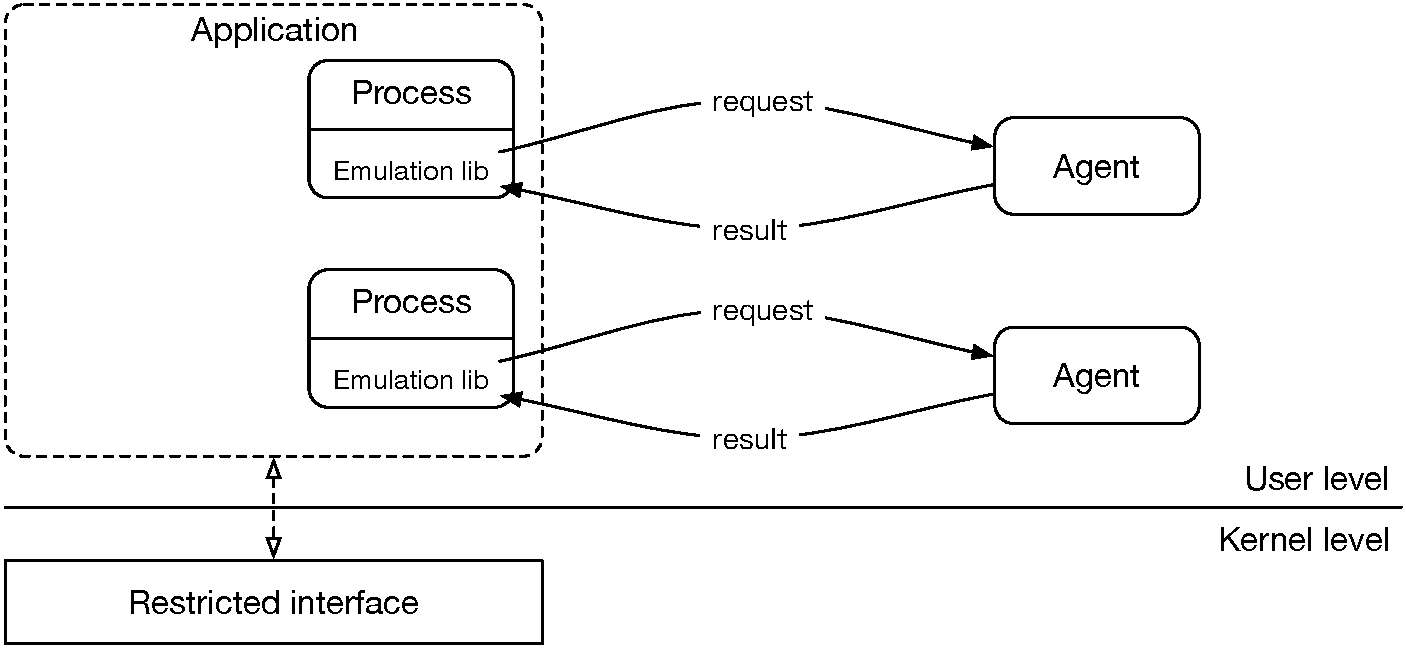
\includegraphics[width=0.8\linewidth]{imgs/ostia}
\caption{Ostia 架构图}
\label{fig:ostia}
\end{figure*}

因此,所有敏感的系统调用,都会被重定向到 agent 中进行处理,这样的架构在 Ostia 中被称为委托代理架构。Ostia 可以解决一部分 Janus 不能解决的数据竞争问题。

\subsection{Software-based Fault Isolation(SFI)}
\label{ss:sfi}

浏览器是一个泛用性很强的应用,因此浏览器要求支持以插件的方式进行功能扩展。同时,为了提高浏览器中代码执行的性能,目前很多浏览器都在探索在浏览器中执行 Native 代码的方法。其中谷歌浏览器支持将 Native 代码运行在一个使用 Software-based Fault Isolation(以下称为 SFI) 的沙箱中。SFI 是在 1994 年在 Wahbe 的论文中第一次出现的 \cite{wahbe1994efficient},SFI 通过修改程序二进制的方式,使得程序的二进制代码符合一些规则,来完成对于错误的隔离。在后来的论文中,谷歌结合了 SFI 和其他的一些沙箱技术,实现了一个面向 Native 代码运行环境的沙箱,这项技术一直到现在仍在被谷歌 Chrome 浏览器使用 \cite{nacl}。

\subsubsection{Efficient Software-based Fault Isolation}
\label{sss:esfi}

Fault Isolation 是一个在计算机科学领域存在已久的定义。在这篇论文发表之前,操作系统已经在软件和硬件层面都进行了 Fault Isolation 的实现。Remote Procedure Call(以下称为 RPC)实现了两个不同的进程间互不影响的通信,而使用不同的虚拟内存空间使得错误不会在两个进程中传播。但是这样的实现中,两个进程进行通信的成本是非常高的。

\begin{figure*}
\centering
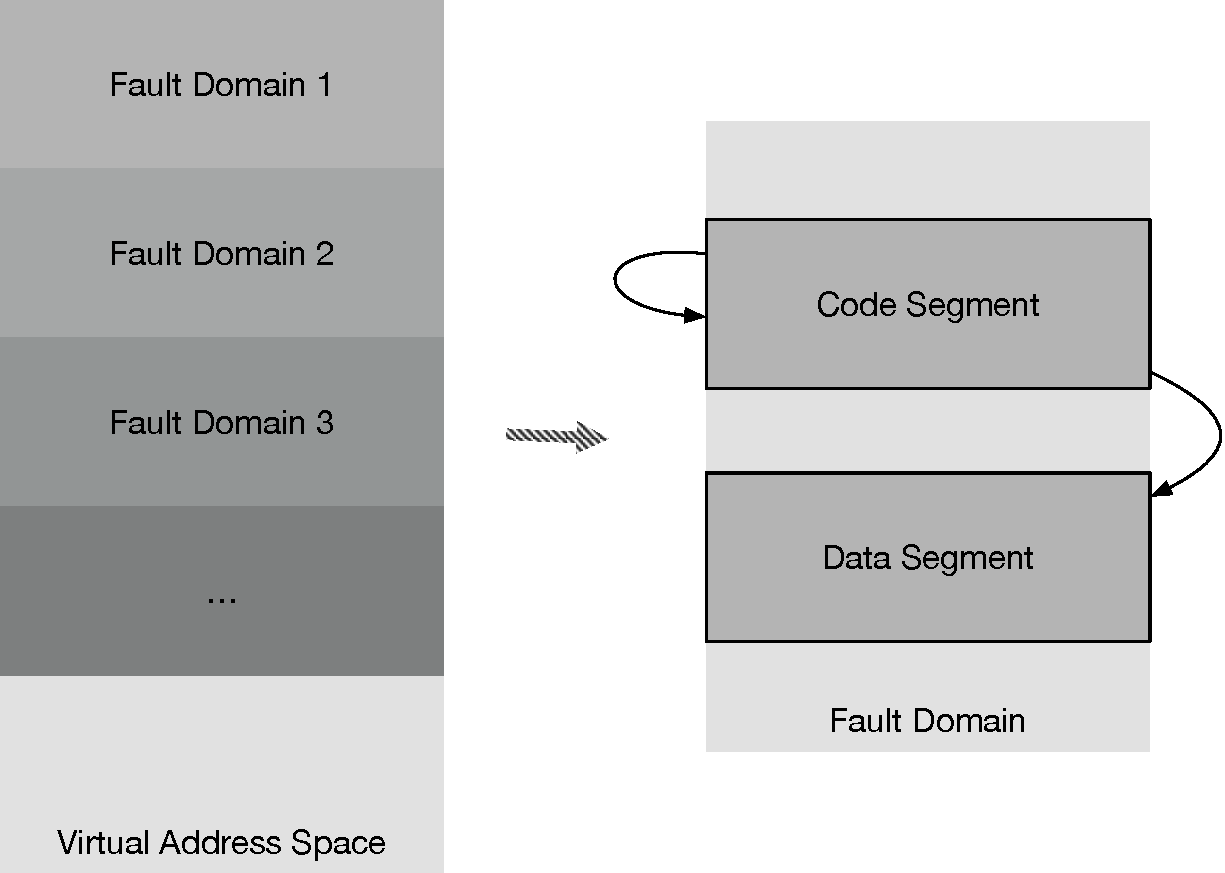
\includegraphics[width=0.8\linewidth]{imgs/sfi}
\caption{Software-based Fault Isolation}
\label{fig:sfi}
\end{figure*}

这一篇论文第一次使用沙箱一词来描述基于软件的错误隔离机制,希望能够在同一地址空间中实现错误的隔离,这样就可以大大减小通信的开销。同一虚拟内存空间被划分成若干个 Fault Domain,每个 Fault Domain 都有自己的数据段和代码段,图 \ref{fig:sfi} 阐述了这篇论文的实现思路,对于每个 Fault Domain 而言,其只能在自己的代码段中进行控制流的转移,与此同时也只能访问自己的数据段 \cite{wahbe1994efficient}。

SFI 的实现,使用了处理器的段寄存器。段寄存器最初是为了解决 Intel 8086 处理器体系架构中数据总线与地址总线的宽度不一致而引入的,因为不一致导致寻址不能在单个指令周期内完成,因此 Intel 引入了段寄存器,将整个内存空间分为了4个段,段寄存器存放每个段的前 N 位的地址,使用段内偏移量,而不是全部的物理地址来描述内存地址,解决了这一问题\footnote{https://en.wikipedia.org/wiki/X86\_memory\_segmentation}。在目前处理器的架构中,不再存在地址宽度不统一的问题,因此内存分段成为了可选的特性。而 SFI 通过对段寄存器的访问限制,将程序的控制流严格地限制在一个 Fault Domain 的代码段中。在进行控制的跳转时,会强制使用段寄存器进行检测,如果访问的地址的前 N 位与段基地址不一致,则会触发异常,说明应用程序正在尝试逃出自己的 Fault Domain。

SFI 的隔离实现,相比于传统的方式有着更小的 overhead,同时也开创了一种新的隔离机制。

\subsubsection{Native Client}
\label{sss:nacl}

Native Client 是谷歌 Chrome 浏览器上的一个特性,开发者可以通过它在浏览器中运行原生的程序,以解决以 Javascript 为代表的浏览器端代码执行效率慢的问题。严格来说 Native Client 结合了 SCI, SFI 等多种技术,进行了实现。

插件程序是各种主流浏览器都有支持的扩展方式,通过插件的方式,用户可以为自己的浏览器增添新的特性与功能。微软的 ActiveX 是最著名的插件支持,在用户浏览网页时,IE 浏览器可以自动下载网页上的 ActiveX 控件,增强网页的功能。但是 ActiveX 也因为漏洞多而饱受争议,所有的控件拥有访问 Windows API 的权力,这使得操作系统的安全受到了很大的挑战。而 Native Client 希望将插件运行在一个隔离可控的沙箱中,用沙箱来限制插件的执行环境。

\begin{figure*}
\centering
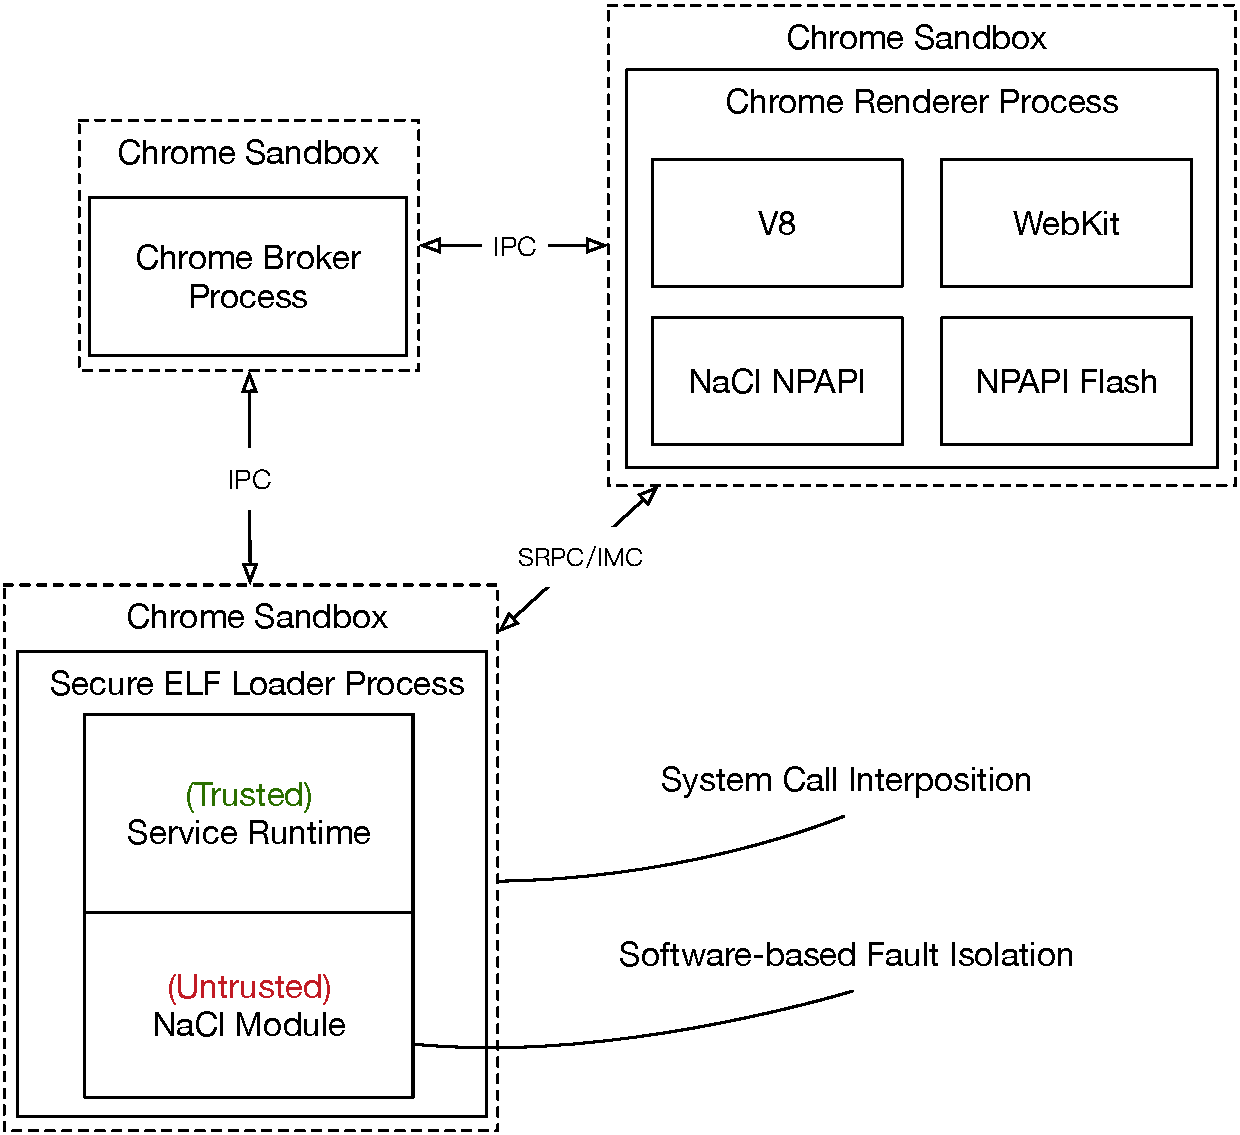
\includegraphics[width=0.65\linewidth]{imgs/nacl}
\caption{Native Client 架构图}
\label{fig:nacl}
\end{figure*}

Native Client 使用了两层沙箱的架构,内层沙箱使用了 SFI 的技术,外层沙箱使用了 SCI 的技术。Native Client 相比于之前的实现,最大的贡献是改进了 SFI 的实现,减小了其在运行时的 overhead。图 \ref{fig:nacl} 中的 Native Client Module,即原生的插件代码。这一部分是通过谷歌修改过的 LLVM 或者 gcc 工具链编译出的二进制程序,在编译时会保证一定的规则,比如在跳转时进行段寄存器的校验等等 SFI 相关的指令检查。这是内层沙箱,这一层沙箱保证了原生的插件代码只能在自己的 Fault Domain 中运行。外层沙箱是由 Systrace \cite{provos2003improving} 提供的类似上文中提到的 Janus 和 Ostia 的系统调用拦截的特性。

在之前的 SFI 实现中,为了在跳转时检查控制流的转移是否合法,需要额外的14个字节的指令。而在 Native Client 中,通过使用对齐的内存,使得跳转指令只能跳转到在32字节对齐的地址段中的第一个地址处。因此,在跳转时的检查由原本的14个字节的指令变成了8个字节的指令。这也是 Native Client 对于之前的研究最大的改进。

\subsection{Capabilities}
\label{ss:capabilities}

// TODO: 加一段浏览器使用场景的引入

早在1988年,Normhardy就提出了confused deputies problem \cite{deputies} 问题,并借此指出了capability的意义与价值。Confused deputies problem的场景可以大致描述为,一个程序需要在执行不同任务的时候,分别取得了不同的权限,这里的权限与前述的任务一一对应,但是一些恶意行为会混淆这里的权限与任务的对应,从而使得程序具有了执行不可预计的行为的权限,即其根本原因在于程序行为与其所拥有的权限之间的映射关系没能被很好的维护。但是在处理这个问题的时候,传统的基于ACL机制的解决方法往往会使得这个维护过程极其复杂,尤其当这里的映射关系的种类和数量变得繁多的时候,哪怕只是更新一个映射,其所带来的边际成本都会是递增的。同时,在这个问题上,"blame the user"(在这里,user是程序本身)是不合理的,而是应该是由OS来应对这个安全问题\footnote{http://wiki.c2.com/?ConfusedDeputyProblem}。Capability作为一种被认为是可行的解决方案,其核心思想是

// TODO: 核心思想 + 可靠(与ACL从效果上一致)

而Capability-based Security由于性能上的问题,大都被OS发行商所拒绝,很少出现在商业化的OS上。Capsicum \cite{capsicum} 作为被纳入FreeBSD的一个基于capability的安全框架,是主要的一种系统级别的实现方式,并被Chromium作为其在FreeBSD下的安全基础\footnote{https://wiki.freebsd.org/Chromium}。下文将以此作为样例,展开阐述capability在系统级实现中的相关细节。

\subsubsection{设计思路}
\label{sss:design}

// TODO: 设计思路 + 涉及到的系统改动
//记得解释 principle of least privilege以及ambient authority

\subsubsection{应用调整}
\label{sss:adoption}

// TODO: 应用的相应调整 + 效果

而实际上,即使不在系统级别上实现capability-based security,依旧可以从编程的角度,进行capability-oriented programming\footnote{http://wiki.c2.com/?CapabilityOrientedProgramming}。

\section{Sandboxing 各种实现的分析与对比}
\label{s:evaluation}

% SFI 只能针对特定平台(ARM,X86)

\begin{figure*}
\centering
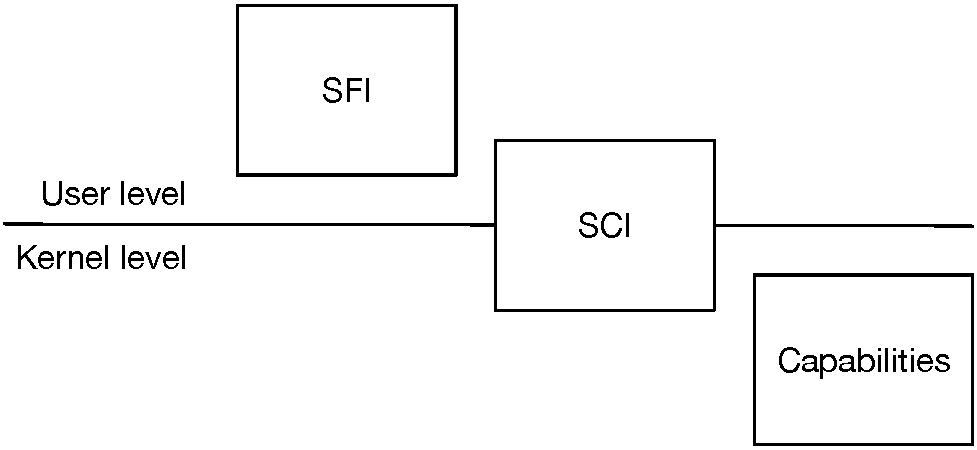
\includegraphics[width=0.7\linewidth]{imgs/difference}
\caption{三种实现的比较}
\label{fig:difference}
\end{figure*}

\section{讨论与总结}
\label{s:tucao}

% 目前 Web Assembly 得到了很大的关注,基本来说 nacl 算是 GG 了,心疼我谷。不过值得一提, Web Assembly 是 nacl 和 asm.js 的团队一起开发出来的。JavaScript 之父 Brendan Eich 曾经在采访中说大概 Wasm 是对 nacl 的最后一击。Web Assembly 上的安全是之后的一个比较有意义的研究方向,因为现在 Wasm 是业界主流,大家都说好,能为它的安全做出一点微小的贡献,不仅有研究意义,还有业界的价值。
% https://my.oschina.net/1pei/blog/488584

\clearpage

\section*{参考文献}

%% The Appendices part is started with the command \appendix;
%% appendix sections are then done as normal sections
%% \appendix

%% \section{}
%% \label{}

%% If you have bibdatabase file and want bibtex to generate the
%% bibitems, please use
%%
%%  \bibliographystyle{elsarticle-num} 
%%  \bibliography{<your bibdatabase>}

%% else use the following coding to input the bibitems directly in the
%% TeX file.

\bibliographystyle{elsarticle-num} 
\bibliography{myref}

\end{document}
\endinput
